\documentclass{article} 
\usepackage{graphicx}
\usepackage[francais]{babel} 
\usepackage[utf8]{inputenc}
\usepackage[T1]{fontenc} 
\usepackage{amsmath} 
\usepackage{amsfonts}
\usepackage{verbatim} 
\usepackage{float} 
\usepackage{hyperref}
\usepackage{scrtime}
\usepackage{Sweave}
\begin{document}
\Sconcordance{concordance:serie1-solutions.tex:/home/francois/ACT-2010-Exercices/serie1-solutions.Rnw:%
1 13 1 1 0 8 1 1 2 1 0 3 1 3 0 1 2 1 1 1 2 20 0 1 8 7 1 1 2 19 0 1 2 1 %
7 7 1 1 2 19 0 1 2 1 7 9 1 1 2 19 0 1 2 1 1 1 2 19 0 1 2 1 1 1 2 19 0 1 %
2 1 1 1 2 1 0 1 1 10 0 1 1 3 0 1 3 19 0 1 2 1 10 7 1 1 2 1 0 2 1 7 0 1 %
2 2 1 1 2 1 0 1 1 3 0 1 2 37 1}


\section{Méthodes de lissage et saisonnalité}
\label{sec:serie-dexercices-1}

\subsection{Noël s'en vient !}
\label{sec:exercice-1-1}


\textbf{Tableau des données}
\begin{Schunk}
\begin{Sinput}
> xtable(Yt.ts,digits=1)
\end{Sinput}
% latex table generated in R 2.15.2 by xtable 1.7-1 package
% Sat Sep 14 23:46:09 2013
\begin{table}[ht]
\centering
\begin{tabular}{rrrrrrrrrrrrr}
  \hline
 & Jan & Feb & Mar & Apr & May & Jun & Jul & Aug & Sep & Oct & Nov & Dec \\ 
  \hline
2008 &  &  &  &  &  &  & 3.4 & 3.5 & 3.4 & 2.6 & 2.0 & 1.2 \\ 
  2009 & 1.1 & 1.4 & 1.2 & 0.4 & 0.1 & -0.3 & -0.9 & -0.8 & -0.9 & 0.1 & 1.0 & 1.3 \\ 
  2010 & 1.9 & 1.6 & 1.4 & 1.8 & 1.4 & 1.0 & 1.8 & 1.7 & 1.9 & 2.4 & 2.0 & 2.4 \\ 
  2011 & 2.3 & 2.2 & 3.3 & 3.3 & 3.7 & 3.1 & 2.7 & 3.1 & 3.2 & 2.9 & 2.9 & 2.3 \\ 
  2012 & 2.5 & 2.6 & 1.9 & 2.0 & 1.2 & 1.5 & 1.3 & 1.2 & 1.2 & 1.2 & 0.8 & 0.8 \\ 
  2013 & 0.5 & 1.2 & 1.0 & 0.4 & 0.7 & 1.2 & 1.3 &  &  &  &  &  \\ 
   \hline
\end{tabular}
\end{table}\end{Schunk}
\textbf{Graphique des données}
\begin{figure}[!ht]
  \centering
  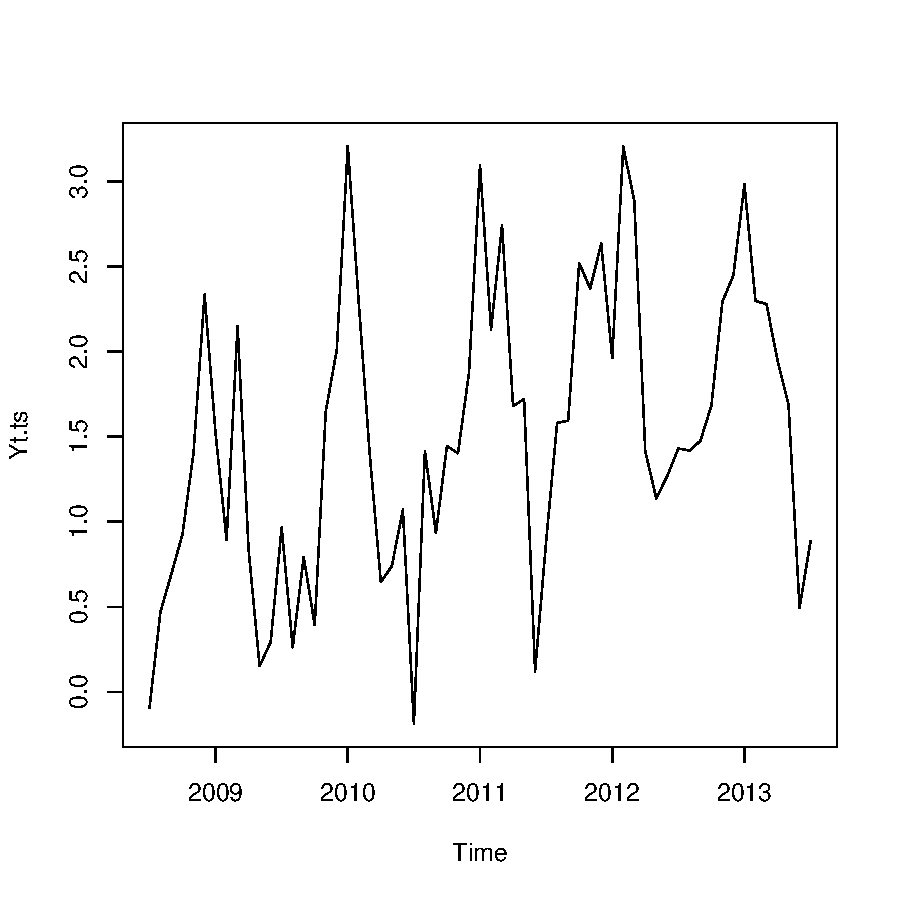
\includegraphics[height=4in, width=4in]{exercice1-graph1.pdf}
  \caption{Graphique de la série $Y_t$}
  \label{fig:exercice1-graph1}
\end{figure}


\clearpage
Document généré le  \today  \ à \ \thistime

\end{document}
